\chapter{Genetic Algorithm}

\textbf{Question:} Simulate one step of Genetic Algorithm (selection, crossover and mutation) for the following function. Represent the population, $x$ using 6 bits. Consider the population size as $F(x) = {2x^2 + 3; 0 \leq x \leq 63}$.


\textbf{Solution:}\\[0.5em]
Initialization,\\
Number of chromosomes = $4$\\
Number of bits/gene in each chromosome = $6$\\
Let, $C1$ : 100011 \quad $C2$ : 110101 \quad $C3$ : 010110 \quad $C4$ : 100100

\vspace{1em}
\textbf{Selection:}\\[0.5em]
\begin{tabularx}{\textwidth}{|l|C|M{2cm}|M{3cm}|c|c|c|}
   \hline
   String no
   & Initial Population
   & $x$ Value
   & Fitness Value $F(x) = {2x^2 + 3}$
   & Probability$_i$
   & Expected Count
   & Actual Count
   \\\hline

   1 & 100011 & 35 & 2453 & 0.21 & 0.84 & 1 \\\hline
   2 & 110101 & 53 & 5621 & 0.48 & 1.93 & 2 \\\hline
   3 & 010110 & 22 & 971 & 0.08 & 0.33 & 0 \\\hline
   4 & 100100 & 36 & 2595 & 0.22 & 0.89 & 1 \\\hline

   Sum &&& 11640 & 1.00 & 4.00 & 4 \\\hline
   Average &&& 2910 & 0.25 & 1.00 & 1 \\\hline
   Max &&& 5621 & 0.48 & 1.93 & 2 \\\hline
\end{tabularx}

\vspace{1em}
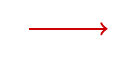
\begin{tikzpicture}
   \pie[
      text=legend,
      radius=2,
      sum=auto,
      after number = ,
      color = {
            red!60,
            blue!40,
            green!50,
            orange!80
      }
   ]
   {21/1 (0.21), 48/2 (0.48), 8/3 (0.08), 22/4 (0.22)}

   \draw[->, thick, red!80!black] (-3,0) -- ++(1,0);
\end{tikzpicture}


\pagebreak
\textbf{Crossover:}\\[0.5em]
\begin{tabularx}{\textwidth}{|l|C|M{3cm}|C|C|C|}\hline
   String no.
   & Mating Pool
   & Crossover Point
   & Offspring
   & $x$ value
   & Fiteness $(2x^2 + 3)$ \\\hline
   1 & 100011 & 3 & 100101 & 37 & 2741 \\\hline
   2 & 110101 & 3 & 110011 & 51 & 5205 \\\hline
   2 & 110101 & 3 & 110100 & 52 & 5411 \\\hline
   4 & 100100 & 3 & 100101 & 37 & 2741 \\\hline
   Sum &&&&& 16098 \\\hline
   Average &&&&& 4024.5 \\\hline
   Max &&&&& 5411 \\\hline
\end{tabularx}

\vspace{1em}
\textbf{Mutation:}\\[0.5em]
\begin{tabularx}{0.8\textwidth}{|l|C|C|M{2cm}|C|}\hline
   String no.
   & Offspring after crossover
   & Offspring after mutation
   & $x$ value
   & Fitness $(2x^2 + 3)$ \\\hline
   1 & 100101 & 110101 & 53 & 5621 \\\hline
   2 & 110011 & 110011 & 51 & 5205 \\\hline
   2 & 110100 & 110100 & 52 & 5411 \\\hline
   4 & 100101 & 110101 & 53 & 5621 \\\hline
   Sum &&&& 21858 \\\hline
   Average &&&& 5464.5 \\\hline
   Max &&&& 5621 \\\hline
\end{tabularx}
